\section{Results}
\label{sec-results}
Table \ref{table-graphsize} reports on the effectiveness of our symmetry breaking
algorithm by measuing the percentage of nodes pruned from each set of maps.
We give figures for the minimum, maximum and average number of nodes pruned
in each of the three benchmarks.
We also give the standard deviation as an indicator for the level of variability
associated with each result.
Meanwhile, in Figure \ref{fig-speedup} we present the average speedup experienced by A* 
when running on our modified grid maps as compared to the original.
We measure speedup in terms of node expansions and search times.
For example, a search time speedup of 2.0 is twice a fast; a node expansion speedup of 2.0 
indicates 50\% fewer nodes were expanded.
We will see that the time speed-up is greater than the node speed-up.
This is because operations for maintaining the open list depend on the size of the list
and thus having a smaller open list makes each such operation faster.

We will discuss our results on each benchmark in turn.
\input graphsize
\textbf{Adaptive Depth:} 
The topography of the maps in this benchmark were favourable for our
symmetry breaking technique.
Our decomposition algorithm was able to identify many large open areas and
pruned between 50.5\% to 62.3\% of all nodes.
Its average performance was just over 57\%. 
We also noticed a 2-3 fold reduction in the average number of nodes expanded 
by A* and a corresponding search time speed up of between 3-4 times.
For very easy problems (those with path lengths $<$ 25) we observed search times 
that were only 3 times faster on average than running A* on the original map. 
By comparison, problems with longer path lengths were solved 3.5 to 4 times faster.
This is as expected; the number of pruned nodes which do not need to be evaluated
will usually grow with the distance from the starting position to the goal
position. In smaller searches there tend to be fewer opportunities to take advantage 
of the pruning enhancement.
%
%Of course this observation assumes the decomposition algorithm is able identify
%symmetric paths in all rooms that appear on the way to the goal.
%Though this is often the case there is no guarantee in general and the performance
%gain experienced by the search algorithm is closely tied to the topography of 
%the map.
\par
\textbf{Baldur's Gate: }
The maps in this benchmark are a mixture of large open areas, sometimes
interspersed with large obstacles, and small to medium rooms connected
by long and narrow corridors.
Performance on this benchmark is quite different from that observed on Adaptive Depth maps.
Though our decomposition algorithm prunes as many as 70\% of all traversable nodes 
on some maps its average performance was only 29\%. 
There was also a reasonably high level variability in the effectiveness of the 
decomposition from one map to the next, as indicated by the standard deviation
of 10.33\%.
A closer investigation revealed that the 45-degree orientation of these maps
resulted in long sequences of increasing clearance values running left-to-right.
This often causes our decomposition algorithm to stop building a room early and build long
skinny rooms which have few interior nodes.
Nevertheless, we observed that the number of nodes expanded by A* improved by a
factor of between 1.5 to 1.8. This corresponds to a search time speed up of between
2 to 2.5 times faster than A* running on the original map.
We expect that these results would improve significantly given a more effective
decomposition algorithm.
\par
\textbf{Rooms:}
The maps in this benchmark were all very similar, comprising of 32$\times$32
rectangular rooms connected by randomly placed entrances.
Each room is of size 7$\times$7 and contains 49 nodes. 
24 of these (or just under 50\%) are interior nodes which we expected would be
pruned.
This was indeed the case: between 46.4\% to 48.1\% of nodes were pruned by 
the decomposition algorithm with an average performance of 47.55\%.
We observed a similar reduction in the number of nodes expanded by A* yielding
search times approximately 2.75 times faster than A* running on the original
maps.
Given rooms with proportionally larger dimensions we would expect to see a
proportionally larger improvement in the performance of A*.
We expect the same is also true as rooms become smaller where in the worst case
there are no interior nodes to prune from any room.

\begin{figure*}[t]
       \begin{center}
                       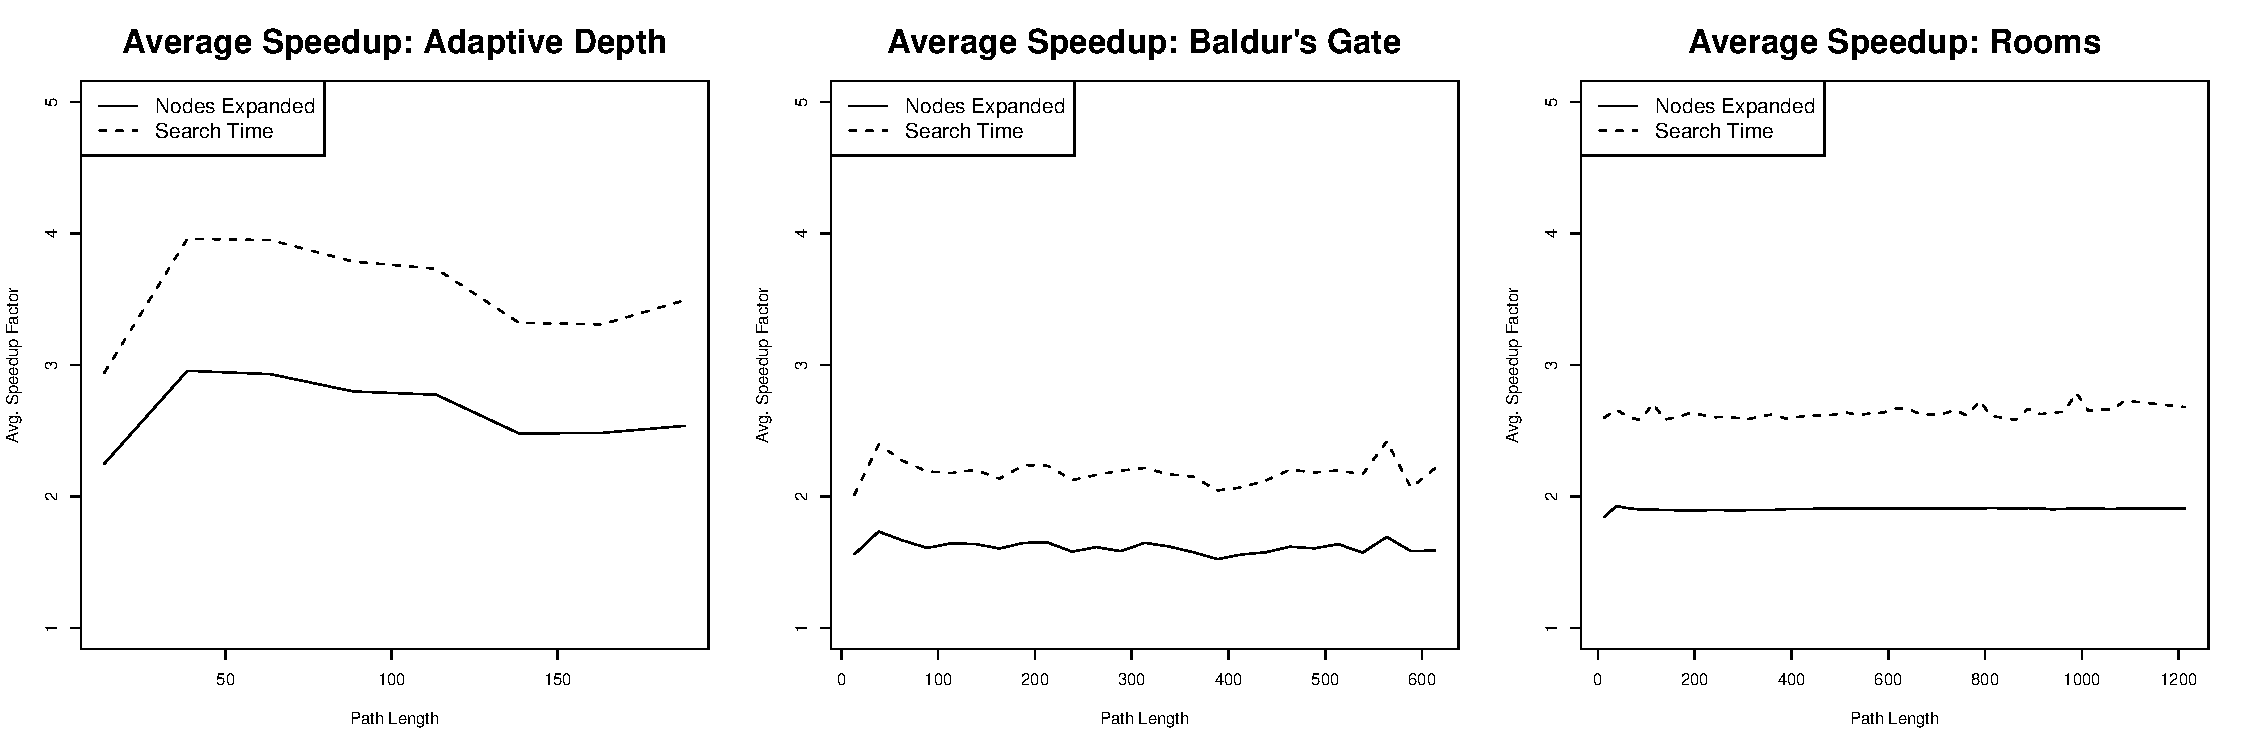
\includegraphics[width=1.95\columnwidth, trim = 10mm 10mm 10mm 0mm]{diagrams/speedup.pdf}
       \end{center}
       \caption{Average A* speedup on each of our three benchmarks. 
		Results are given in terms of nodes expanded and search time.}
\label{fig-speedup}
\end{figure*}
